\section{Διαδικασία μέτρησης και αποτελέσματα}
\subsection{$v_{tacho}$}
Αρχικά, συνδέουμε τον παλμογράφο όπως φαίνεται στο σχήμα~\ref{fig:circuit-1}.
\begin{figure}[htb]
    \centering
    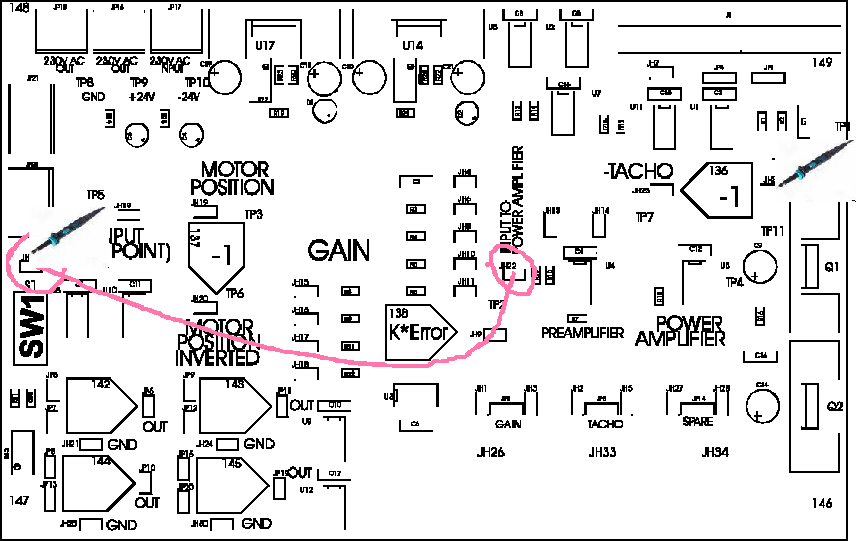
\includegraphics[width=\linewidth]{circuit-1}
    \caption{Σύνδεση παλμογράφου}
    \label{fig:circuit-1}
\end{figure}
Ρυθμίζουμε τον παλμογράφο σε κατάλληλες τιμές \texttt{volt/div} και \texttt{second/div}
και κατάλληλες θέσεις \texttt{X-POS}, \texttt{Y-POS} έτσι ώστε να ``χωράει'' όλη η καμπύλη σε μια οθόνη.
Μετακινούμε το \texttt{SW1} στη θέση των $\SI{+10}{\volt}$.
Περιμένουμε μέχρι να φτάσει η ταχογεννήτρια στη μόνιμή της κατάσταση και πατάμε το κουμπί \texttt{HOLD} ώστε να αποθηκευτεί η καμπύλη στη μνήμη του παλμογράφου.
Μετρούμε είσοδο $U = \SI{10}{\volt}$ και μετακινούμε το \texttt{SW1} στη μεσαία θέση.
Χρησιμοποιώντας τα cursors του παλμογράφου μετράμε την μέγιστη τιμή της τάσης $v_{tacho} = \SI{8.79}{\volt}$.

\subsection{$k_m k_T$}
Για τη συνάρτηση μεταφοράς ισχύει
\begin{equation*}
    \frac{k_m k_T}{T_m s + 1} = k_m k_T
\end{equation*}
όμως στη μόνιμη κατάσταση $s = 0$ και έτσι
\begin{equation*}
    k_m k_T = \frac{v_{tacho}}{U} = 0.879
\end{equation*}

\subsection{$T_m$}
Για τον υπολογισμό της σταθεράς χρόνου $T_m$ μετράμε το χρόνο στον οποίο η καμπύλη φτάνει το $\SI{63.3}{\percent}$ της μέγιστης τιμής της, δηλαδή στη τιμή $0.633 v_{tacho} = \SI{5.56}{\volt}$.
Μειώνουμε το μέγιστο οριζόντιο cursor του παλμογράφου μέχρι να φτάσουμε την επιθυμητή τιμή.
Εκεί, θέτουμε τα cursor του παλμογράφου κατακόρυφα και μετράμε τη διαφορά χρόνου $T_m = \SI{0.641}{\second}$.

\subsection[$k_{μ}$]{$k_{\mu}$}
Μετράμε ότι για μια πλήρη στροφή του δισκόφρενου ο άξονας εξόδου περιστρέφεται κατά $10^{\circ}$.
Άρα $k_{\mu} = \frac{10}{360} = \frac{1}{36}$.

\newcommand{\texodou}{T_{εξ\acute{ο}δου}}
\subsection{$\omega$}
Συνδέουμε τον παλμογράφο όπως φαίνεται στο σχήμα~\ref{fig:circuit-2}.
\begin{figure}[htb]
    \centering
    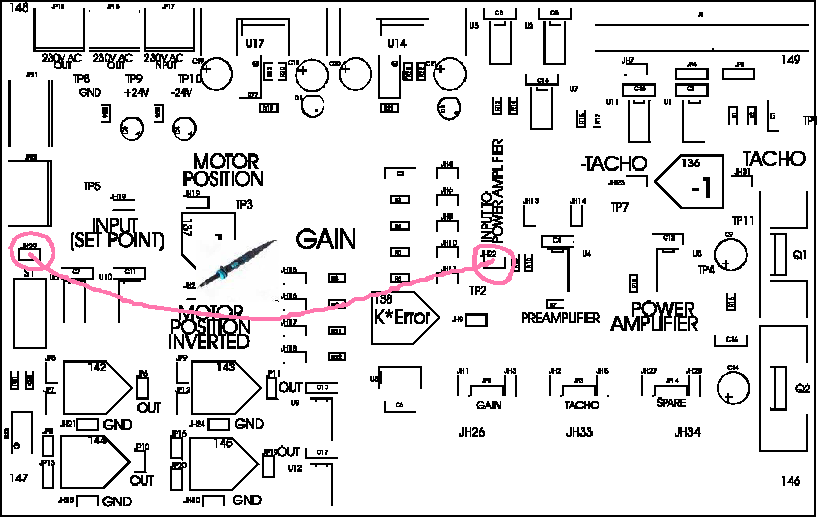
\includegraphics[width=\linewidth]{circuit-2}
    \caption{Σύνδεση παλμογράφου}
    \label{fig:circuit-2}
\end{figure}
Μετακινούμε το \texttt{SW1} στη θέση των $\SI{+10}{\volt}$.
Από τη τριγωνική κυματομορφή που προκύπτει μετράμε τη κλίση και τη διάρκειά της με τη βοήθεια του \texttt{HOLD} και των cursor του παλμογράφου όπως και πριν.
Μετράμε $\SI{0.916}{\second}$ που αντιστοιχούν σε $36$ στροφές άρα η ταχύτητα είναι
$\omega = \SI{2358}{\rpm}$.
Μετακινούμε το \texttt{SW1} στη μεσαία θέση.

\subsection{$k_0$}
Η μεταβολή της θέσης σε volt που μετρήθηκε προηγουμένως είναι $\SI{14}{\volt}$.
Ισχύει:
\begin{equation*}
\frac{\Delta V}{\Delta t} = \omega k_{\mu} k_0 \implies k_0 = \frac{\Delta V}{\Delta t} \frac{1}{\omega k_{\mu}} \implies k_0 = 0.233
\end{equation*}

\subsection{$k_T$}
Ισχύει:
\begin{equation*}
v_{tacho} = K_T \omega \implies k_T = \frac{v_{tacho}}{\omega} = 0.006472
\end{equation*}

\subsection{$k_m$}
Ισχύει:
\begin{equation*}
k_m k_T = 0.879 \implies k_m = 135.8
\end{equation*}

\subsection{${V_{ref}}_{arduino}$ και $V_{7805}$}
Πραγματοποιούμε τη σύνδεση με το arduino και μετράμε (με το \texttt{SW1} ακόμα στη μεσαία θέση) τις 2 καταστάσεις του κινητήρα.
\begin{code}
\begin{minted}{MATLAB}
a = arduino(port);
velocity = analogRead(a,3);
position = analogRead(a,5);
\end{minted}
\end{code}
Προκύπτει \mintinline{MATLAB}!velocity = 565! και \mintinline{MATLAB}!position = 709!.
Μετράμε τη τάση στο pin Motor Position $\SI{10.41}{\volt}$.
Έτσι, οι τιμές που προκύπτουν είναι:
\begin{align*}
{V_{ref}}_{arduino} &= \frac{10.41 \cdot{} 1024}{3 \cdot{} 709} = \SI{5.012}{\volt} \approx \SI{5}{\volt}\\
V_{7805} &= \frac{2 \cdot{} 565 \cdot{} 5.011}{1024} = \SI{5.53}{\volt}
\end{align*}

Με δεύτερες μετρήσεις
(\mintinline{MATLAB}!velocity = 565!, \mintinline{MATLAB}!position = 737! και $\SI{10.7}{\volt}$)
επιβεβαιώνω ότι το ${V_{ref}}_{arduino}$ παίρνει τιμές κοντά στη περιοχή των $\SI{5}{\volt}$ ενώ το $V_{7805}$ παίρνει τιμές κοντά στη περιοχή των $\SI{5.5}{\volt}$.
